\chapter{Performance Evaluations}\label{chap:performance}

\section{Data Preparation and Experiment Setup}
% \subsection{Data and Experiment Setup}
Figure~\ref{fig:input-data} shows the initial P-wave of three axes used in the Multi ES-ELM model. In this research, the data sets are provided by the Taiwan earthquake station network from \cite{chiang2022neural}.
The data are recorded from the CWBSN network from 2014 to 2019 with 896 events and the TSMIP network from 1991 to 2019 with 724 events. They consist of $N = 10,377$ samples of ground motion data and are split into training data $N_{training} = 6,900$ and testing data $N_{testing} = 3,477$ where $T = 500$ (5 seconds after finding P-wave). The data are prescribed for $T = 500$ because this $T$ is the best practice for conventional models \cite{chiang2022neural}.

\begin{figure}[ht]
\centering
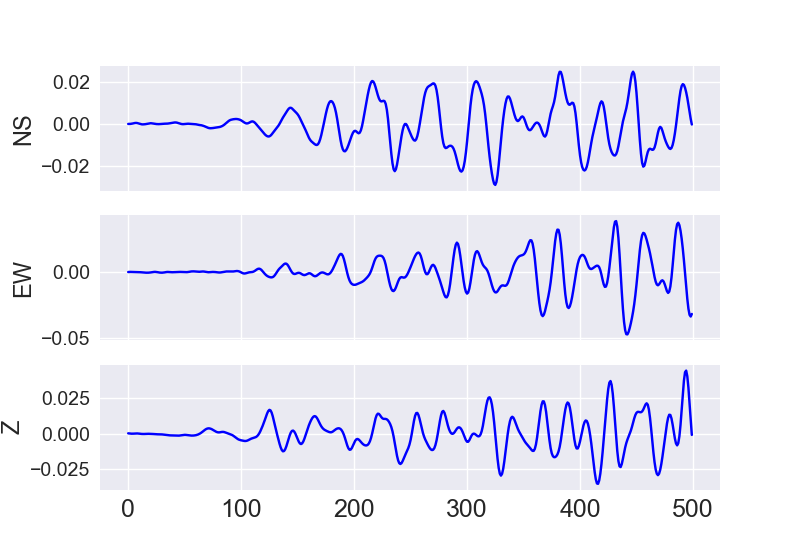
\includegraphics[width=0.9\textwidth]{img/3-axis.png}
\caption{Initial P-wave.} \label{fig:input-data}
\end{figure} 

% {Initial P-wave.\label{input-data}}
The labels of datasets are encoded by one hot encoder. If the PGA of the signal $X_i$ less than $80Gal$ then setting $y_i = [1, 0]$. Otherwise, $y_i = [0, 1]$.

\section{Model evaluation}
The Earthquake Early Warning systems are the systems that classify whether a seismic wave can generate strong motion or not. So, the metrics used in this research need the metrics for the binary classification problem\cite{chiang2022neural}. The most used metric for binary classification is accuracy. 

The outcomes of the model can be represented by four classes. 
\begin{enumerate}
    \item True Positive (TP)\\
    The true positives are the results where the model correctly predicts strong motion. 

    \item False Positive (FP)\\
    The false positives are the results where the model incorrectly predicts strong motion. The model predicts the signals are weak but strong.

    \item True Negative (TN)\\
    The true negative is the result where the model correctly predicts not strong motion (weak motion).

    \item False Negative (FN)\\
    True false negatives are the results where the model incorrectly predicts not strong motion (weak motion). The model predicts the signals are strong but weak.
\end{enumerate}

Furthermore, the four possible outcomes of the model can be visualized in the confusion matrix depicted in Figure \ref{fig:conf-mat}.
\begin{figure}[b]
    \centering
    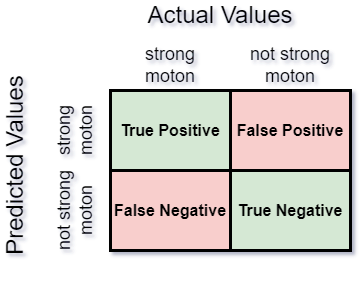
\includegraphics[width=0.7\textwidth]{img/binary-conf-mat.png}
    \caption{The confusion matrix}
    \label{fig:conf-mat}
\end{figure}

However, accuracy is the default metric for classification problems. However, this metric is not the best for imbalanced data like the severity scale of
ground motions. So, the proposed model needs to be measured by other metrics such as precision, true positive rate, and f1-score.

 Precision is the metric that measures how many false positives (or false alerts). So, the high precision leads to fewer false alerts in the system. True positive rate or recall is the metric for showing the ability to detect dangerous events in the system. In other words, high recall means less false negative and high true positive. f1-score is the metric that combines recall and precision.  
 
\subsubsection{accuracy}
The accuracy measures the proportion between correct prediction results (the number of true positives and true negatives) and the total number of data. Which can be expressed as:
$$\text{accuracy} = \frac{TP + TN}{TP + TN + FP + FN}\times 100$$

\subsubsection{precision}
The precision focuses on positive predictions (true positive and false positive). The precision is the ratio of true positive and total all positive observations which can be expressed as:
$$\text{precision} = \frac{TP}{TP + FP}\times 100$$

\subsubsection{recall}
The recall focuses on actual positive observations (true positive and false negative). The recall is the proportion between true positive prediction and all positive observations which can be expressed as:
$$\text{recall} = \frac{TP}{TP + FN}\times 100$$

A higher true positive rate indicates the model can identify the strong motion well.

\subsubsection{f1-score}
The f1-score is the mean between the precision metric and the recall metric  which can be expressed as:
$$\text{f1-score} = 2 \times \frac{\text{precision} \times \text{true positive rate}}{\text{precision} + \text{true positive rate}}\times 100$$

Where $TP, TN, FP,\ $ and $FN$ are true positive, true negative, false positive, and false negative respectively.
\section{Computational Metrics}
The EEW systems necessitate the implementation of an efficient model that facilitates rapid re-training, thereby minimizing the computational resources and time required for this process. This efficiency in re-training is crucial for ensuring the system's responsiveness to changing data and real-time seismic activity monitoring, contributing to the overall effectiveness of the EEW system.
\subsection{Memory usages}
Memory consumption becomes a critical factor during the model training process. Deep learning frameworks like PyTorch involve the transfer of feature vectors between various layers when training a model, necessitating the utilization of temporary memory or RAM. If the training process demands a substantial amount of memory, it often calls for a high-performance computing setup, which, in turn, results in increased operational costs. So, memory usage is an essential metric for assessment in the EEW systems.

PyTorch API provides a module called PyTorch Profile for monitoring the memory usage in the training process. For each process, the module can monitor how much the process consumes the memories and save results in a CSV file. The memories are provided in the megabit (Mb) unit. However, the Deep learning model requires more than a gigabit (GB). Therefore, the results are changed from Mb to GB.

\subsection{Time for training}
Deep learning models designed for processing streaming data, such as seismic waves, encounter a challenge when it comes to real-time model updates. This challenge is due to the time-consuming of the models training process, which obstructs their ability to adapt rapidly to evolving data. So, the training time is a crucial measurement that needs to be observed when using the deep learning models in the EEW systems.

\section{Parameter Optimization}
This section investigates the parameter optimization that is finding the best number of internal units $(W_{input})$ for the EEW model.

% accuracy, true_positive_rate, precision, f1_score
Figures \ref{fig:accuracy}, \ref{fig:true_positive_rate}, \ref{fig:precision}, and \ref{fig:f1score} show the test performance of the Multi ES-ELM model. Increasing the number of internal units could improve the accuracy, precision, and f1-score in some internal unit ranges (5-35 units). However, the models that used more than $35$ internal units had to decrease performances. In addition, true positive rates of the Multi ES-ELM model reduced over the number of internal units.

From the figures \ref{fig:accuracy}, \ref{fig:true_positive_rate}, \ref{fig:precision}, and \ref{fig:f1score}, the smallest internal units that had high performance is $20$. Thus, in the experiment section, the internal unit parameter was set by $20$.

% \Figure[t](topskip=0pt, botskip=0pt, midskip=0pt)[width=0.93\textwidth]{img/time_mem.png}{Time and memory usages.\label{Time for training}}

% \Figure(topskip=0pt, botskip=0pt, midskip=0pt)[width=0.47\textwidth]{img/Accuracy.png}
% {Accuracy.\label{accuracy}}
% \Figure(topskip=0pt, botskip=0pt, midskip=0pt)[width=0.47\textwidth]{img/True positive rate.png}
% {True positive rate (recall).\label{true_positive_rate}}
% \Figure(topskip=0pt, botskip=0pt, midskip=0pt)[width=0.47\textwidth]{img/Precision.png}
% {Precision.\label{precision}}
% \Figure(topskip=0pt, botskip=0pt, midskip=0pt)[width=0.47\textwidth]{img/F1 score.png}
% {F1-score.\label{f1_score}}



% Figure \ref{img/fig4} shows the test performance of the RC model. Increasing the number of internal units cloud improve the accuracy, precision, and f1-score in some internal unit ranges ($5-35$ units). However, the models that used more than $35$ internal units had the decreasing performances. In addition, true positive rates of RC model reduced over the number of internal units.\\

% From the figure \ref{img/fig4}, the smallest internal units that had high performance is $20$. Thus, in experiment section, The internal unit parameter was set by $20$.


% \Figure[t!](topskip=0pt, botskip=0pt, midskip=0pt)[width=5.5 cm]{img/accuracy.png}
% {Accuracy.\label{accuracy}}
% \Figure[t!](topskip=0pt, botskip=0pt, midskip=0pt)[width=5.5 cm]{img/true_positive_rate.png}
% {True positive rate.\label{true_positive_rate}}
% \Figure[t!](topskip=0pt, botskip=0pt, midskip=0pt)[width=5.5 cm]{img/precision.png}
% {Precision.\label{precision}}
% \Figure[t!](topskip=0pt, botskip=0pt, midskip=0pt)[width=5.5 cm]{img/f1_score.png}
% {F1 score.\label{f1_score}}

% \begin{figure}[h]
%     \centering
%     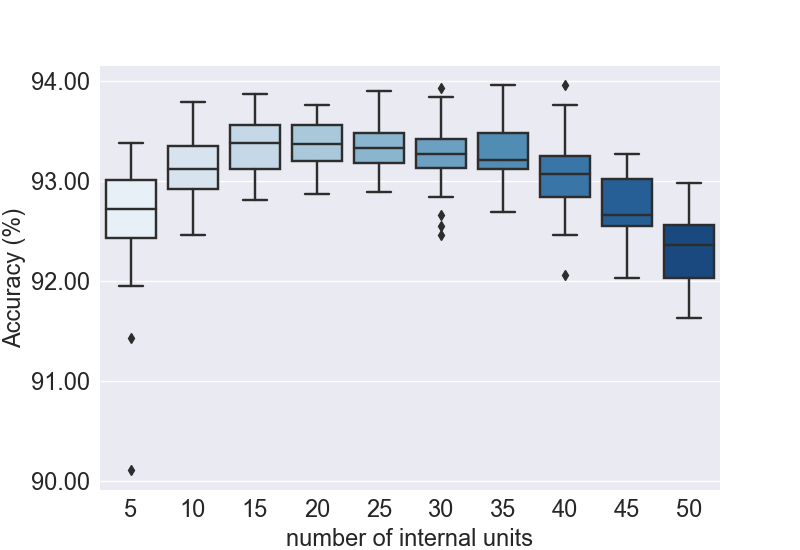
\includegraphics[width=0.5\textwidth]{img/accuracy.png}
%     \caption{Caption}
%     \label{fig:enter-label}
% \end{figure}

% \begin{figure}[h]
%     \centering
%     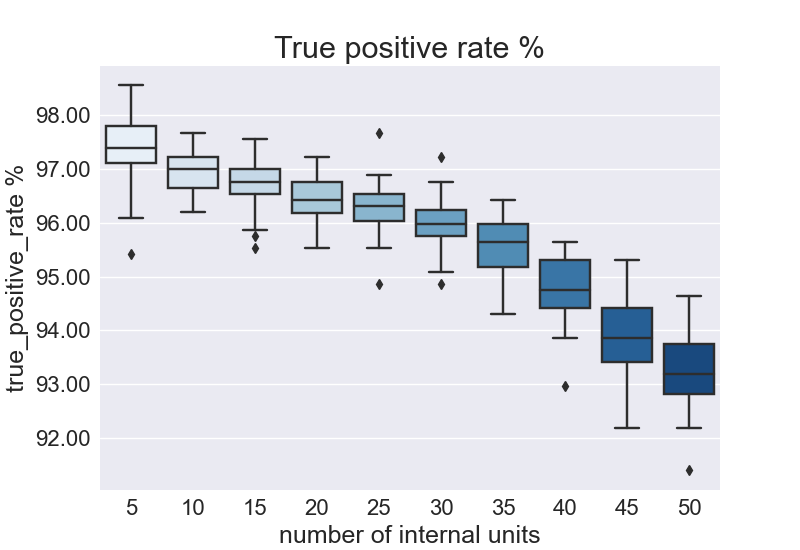
\includegraphics[width=0.5\textwidth]{img/true_positive_rate.png}
%     \caption{Caption}
%     \label{fig:enter-label}
% \end{figure}

% \begin{figure}[h]
%     \centering
%     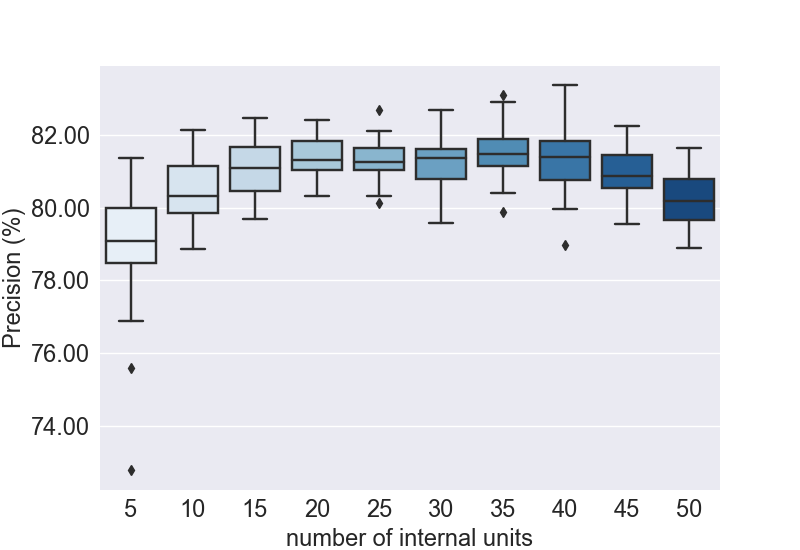
\includegraphics[width=0.5\textwidth]{img/precision.png}
%     \caption{Caption}
%     \label{fig:enter-label}
% \end{figure}

% \begin{figure}[h]
%     \centering
%     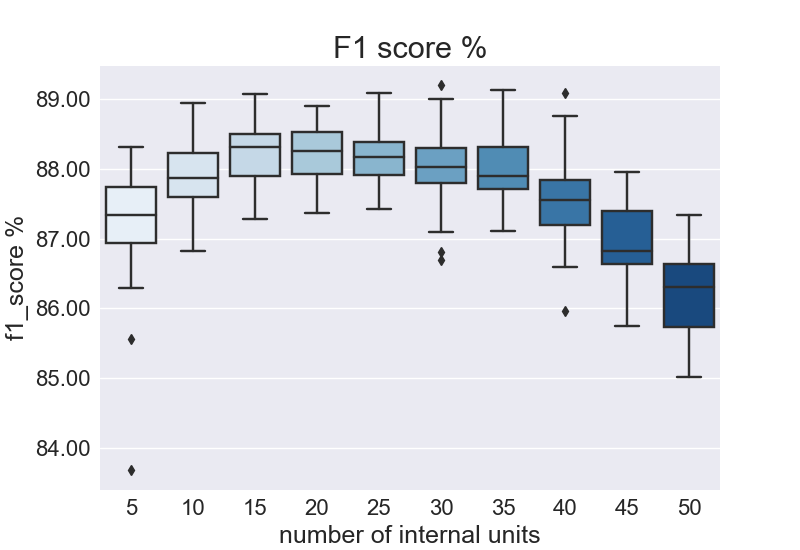
\includegraphics[width=0.5\textwidth]{img/f1_score.png}
%     \caption{Caption}
%     \label{fig:enter-label}
% \end{figure}
\begin{multicols}{2}
\begin{figure}[H]
    \centering
    \begin{subfigure}[b]{0.6\textwidth}
        \centering
        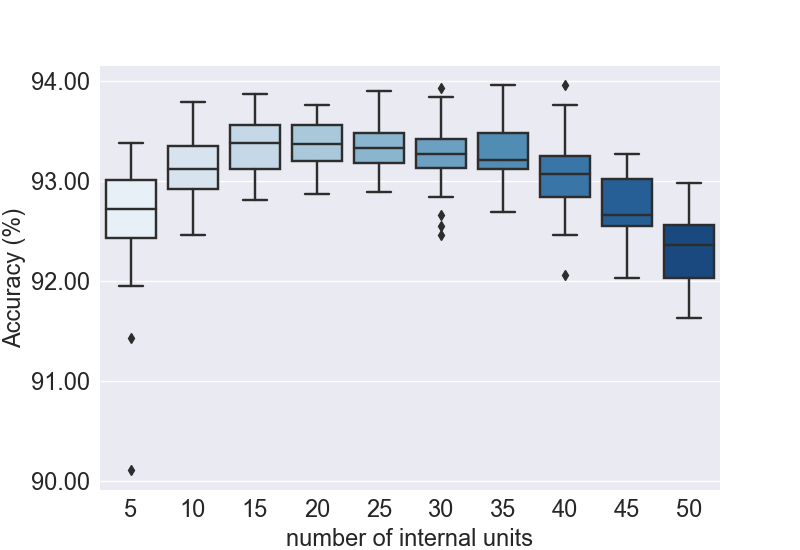
\includegraphics[width=0.8\textwidth]{img/accuracy.png}
        \caption{Accuracy}
        \label{fig:accuracy}
    \end{subfigure}
    \begin{subfigure}[b]{0.6\textwidth}
        \centering
        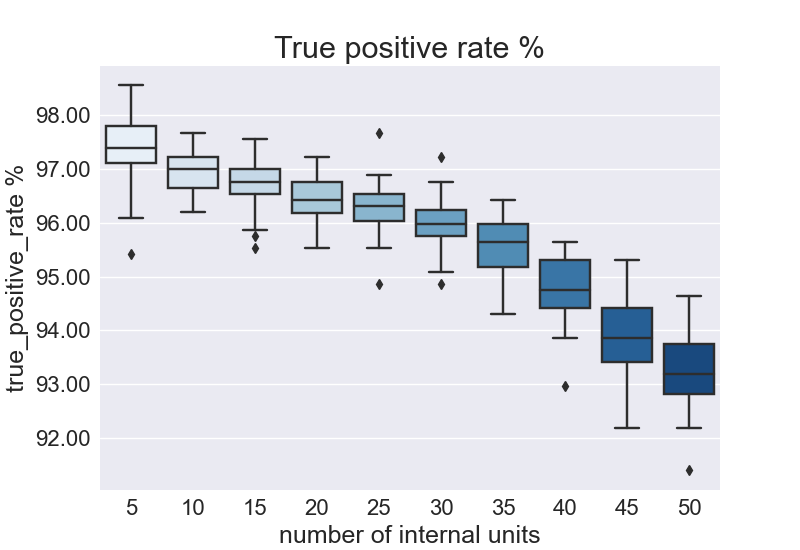
\includegraphics[width=0.8\textwidth]{img/true_positive_rate.png}
        \caption{True positive rate.}
        \label{fig:true_positive_rate}
    \end{subfigure}
\end{figure}

\begin{figure}[H]
    \centering
    \begin{subfigure}[b]{0.6\textwidth}
        \centering
        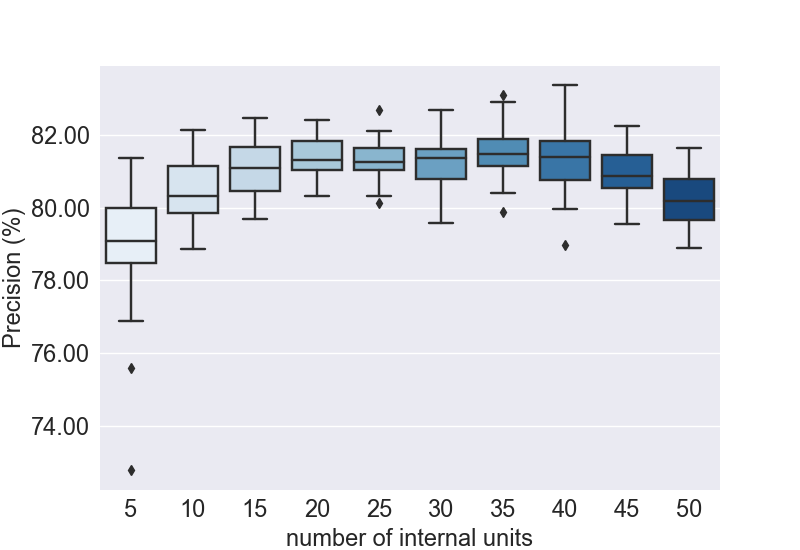
\includegraphics[width=0.8\textwidth]{img/precision.png}
        \caption{Precision.}
        \label{fig:precision}
    \end{subfigure}
    \begin{subfigure}[b]{0.6\textwidth}
        \centering
        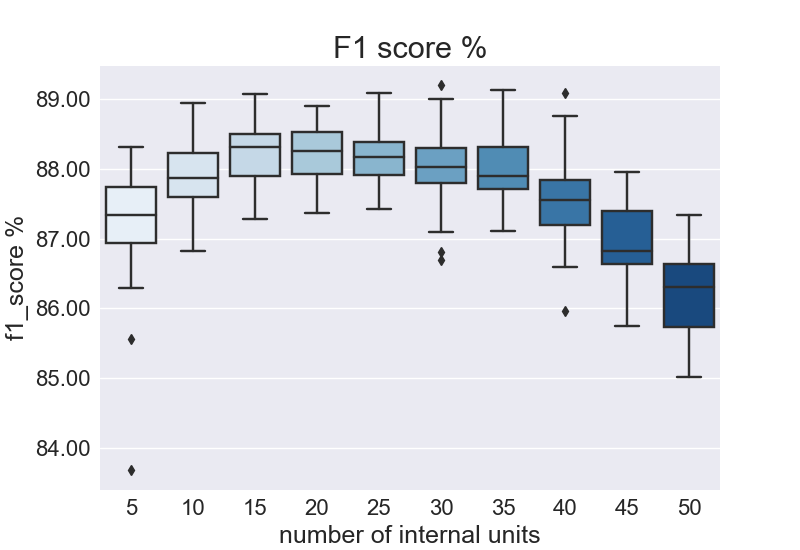
\includegraphics[width=0.8\textwidth]{img/f1_score.png}
        \caption{F1 score.}
        \label{fig:f1score}
    \end{subfigure}
\end{figure}
\end{multicols}


% \Figure[ht](topskip=0pt, botskip=0pt, midskip=0pt)[width=15 cm]{img/mem_time.png}{Time and memory usages.\label{Time for training}}
